\documentclass[aspectratio=169,12pt,t]{beamer}

% --- Theme: Metropolis (modern, clean) ---
\usetheme[progressbar=frametitle,numbering=fraction,block=fill]{metropolis}

% --- Fira Sans font (install texlive-fonts-extra if missing) ---
\IfFileExists{FiraSans.sty}{\usepackage[sfdefault]{FiraSans}}{}

% --- Light background with warm accent ---
\definecolor{mDarkTeal}{RGB}{35,55,59}
\definecolor{mLightBrown}{RGB}{235,228,216}
\definecolor{mAccent}{RGB}{140,70,20}

\setbeamercolor{normal text}{fg=mDarkTeal,bg=white}
\setbeamercolor{alerted text}{fg=mAccent}
\setbeamercolor{frametitle}{bg=mDarkTeal,fg=white}
\setbeamercolor{progress bar}{fg=mAccent,bg=mLightBrown}
\setbeamercolor{title separator}{fg=mAccent}
\setbeamercolor{progress bar in head/foot}{fg=mAccent,bg=mLightBrown}
\setbeamercolor{progress bar in section page}{fg=mAccent,bg=mLightBrown}

% --- Packages ---
\usepackage[utf8]{inputenc}
\usepackage{amsmath,amssymb,amsthm}
\usepackage{mathrsfs}
\usepackage{tikz}
\usetikzlibrary{arrows.meta,positioning,calc,decorations.pathreplacing,shapes,patterns}
\usepackage{pgfplots}
\pgfplotsset{compat=1.18}

% --- Custom colors for content types ---
\definecolor{defcolor}{RGB}{25,85,120}
\definecolor{thmcolor}{RGB}{140,35,35}
\definecolor{proofcolor}{RGB}{35,100,50}
\definecolor{excolor}{RGB}{140,75,10}
\definecolor{remcolor}{RGB}{90,90,90}

% --- Beamer blocks for mathematical content types ---
\newenvironment{defblock}[1]{%
  \setbeamercolor{block title}{bg=defcolor,fg=white}%
  \setbeamercolor{block body}{bg=defcolor!5}%
  \begin{block}{#1}}{\end{block}}

\newenvironment{thmblock}[1]{%
  \setbeamercolor{block title}{bg=thmcolor,fg=white}%
  \setbeamercolor{block body}{bg=thmcolor!5}%
  \begin{block}{#1}}{\end{block}}

\newenvironment{proofblock}[1]{%
  \setbeamercolor{block title}{bg=proofcolor,fg=white}%
  \setbeamercolor{block body}{bg=proofcolor!5}%
  \begin{block}{#1}}{\end{block}}

\newenvironment{exblock}[1]{%
  \setbeamercolor{block title}{bg=excolor,fg=white}%
  \setbeamercolor{block body}{bg=excolor!5}%
  \begin{block}{#1}}{\end{block}}

\newenvironment{remblock}[1]{%
  \setbeamercolor{block title}{bg=remcolor,fg=white}%
  \setbeamercolor{block body}{bg=remcolor!5}%
  \begin{block}{#1}}{\end{block}}

% --- Metadata ---
\title{Principles of Mathematical Analysis}
\subtitle{Preface: About This Series}
\author{Based on Walter Rudin's \emph{Principles of Mathematical Analysis}}
\date{}

\begin{document}

% ============================================================
% TITLE
% ============================================================
\begin{frame}
  \titlepage

  \note{
    Welcome to the Principles of Mathematical Analysis video series. Before we dive into the mathematics, let's take a moment to talk about what this series is, where the material comes from, and how you can get the most out of it.
  }
\end{frame}

% ============================================================
\begin{frame}{Outline}
  \tableofcontents

  \note{
    Here is what we will cover in this short preface. First, we will give proper credit to the source material. Then we will explain the goals of the series. After that, we will walk through the complete list of chapters, so you know what to expect. Finally, we will talk about how this project is open source and how you can contribute. Let's begin.
  }
\end{frame}

% ============================================================
\section{Credit and Source}
% ============================================================

% --- Build 1/3 ---
\begin{frame}{About the Source Material}
  \begin{remblock}{Based on a classic text}
    This series is based on Walter Rudin's\\
    \alert{\emph{Principles of Mathematical Analysis}}\\
    (commonly known as ``Baby Rudin'').
  \end{remblock}

  \note{
    This entire video series is based on the classic textbook Principles of Mathematical Analysis by Walter Rudin. Among mathematicians, this book is affectionately known as Baby Rudin, to distinguish it from Rudin's other, more advanced book Real and Complex Analysis. It has been a standard reference for undergraduate and early graduate analysis for more than half a century.
  }
\end{frame}

% --- Build 2/3 ---
\begin{frame}{About the Source Material}
  \begin{remblock}{Based on a classic text}
    This series is based on Walter Rudin's\\
    \alert{\emph{Principles of Mathematical Analysis}}\\
    (commonly known as ``Baby Rudin'').
  \end{remblock}

  \vspace{0.5em}
  \textbf{All credit for the mathematical content} goes to Walter Rudin and his publisher.

  \note{
    All credit for the mathematical content, the definitions, the theorems, the proofs, and the overall structure goes to Walter Rudin and his publisher. This series does not replace the book. It is a companion to it. We are simply re-presenting the material in a new format, with visuals and narration, to help learners engage with it more easily.
  }
\end{frame}

% --- Build 3/3 ---
\begin{frame}{About the Source Material}
  \begin{remblock}{Based on a classic text}
    This series is based on Walter Rudin's\\
    \alert{\emph{Principles of Mathematical Analysis}}\\
    (commonly known as ``Baby Rudin'').
  \end{remblock}

  \vspace{0.5em}
  \textbf{All credit for the mathematical content} goes to Walter Rudin and his publisher.

  \vspace{0.5em}
  \alert{Please use the book as your primary reference.}

  \note{
    If you are serious about learning analysis, please buy a copy of the book and use it as your primary reference. These videos are designed to walk alongside the book, not to replace it. Reading the original text is still the best way to absorb the precision and elegance of Rudin's writing.
  }
\end{frame}

% ============================================================
\section{Goals of This Series}
% ============================================================

% --- Build 1/4 ---
\begin{frame}{Why This Series Exists}
  \textbf{Goal:} Make mathematical analysis\\
  \alert{easier and more accessible}.

  \note{
    Rudin's book is famous for its beauty, but also for its terseness. Proofs are compact, intuition is often left to the reader, and there are almost no pictures. The goal of this series is simple: to make the material easier and more accessible, without losing any of the mathematical rigor.
  }
\end{frame}

% --- Build 2/4 ---
\begin{frame}{Why This Series Exists}
  \textbf{Goal:} Make mathematical analysis\\
  \alert{easier and more accessible}.

  \vspace{0.5em}
  \begin{itemize}
    \item \alert{Additional insights} and motivation behind each result
  \end{itemize}

  \note{
    To do this, each slide comes with additional insights and motivation. We try to explain why a definition is made the way it is, what problem a theorem is really solving, and why a proof takes the particular shape it does. These are the kinds of things an experienced mathematician knows, but that are not always written down in the book.
  }
\end{frame}

% --- Build 3/4 ---
\begin{frame}{Why This Series Exists}
  \textbf{Goal:} Make mathematical analysis\\
  \alert{easier and more accessible}.

  \vspace{0.5em}
  \begin{itemize}
    \item \alert{Additional insights} and motivation behind each result
    \item \alert{Diagrams} and visualizations (the book has none!)
  \end{itemize}

  \note{
    We also add diagrams and visualizations throughout. The original book contains essentially no figures, which is a missed opportunity because many ideas in analysis are deeply geometric. Number lines, epsilon neighborhoods, function graphs, compact covers, and convergence pictures can all make abstract statements suddenly click.
  }
\end{frame}

% --- Build 4/4 ---
\begin{frame}{Why This Series Exists}
  \textbf{Goal:} Make mathematical analysis\\
  \alert{easier and more accessible}.

  \vspace{0.5em}
  \begin{itemize}
    \item \alert{Additional insights} and motivation behind each result
    \item \alert{Diagrams} and visualizations (the book has none!)
    \item \alert{Progressive builds}: one idea at a time
  \end{itemize}

  \note{
    Finally, the slides use progressive builds, which means ideas are revealed one at a time. This matches the pace of a video lecture and gives you a chance to absorb each step before the next one appears. The idea is that you can follow along naturally, without feeling overwhelmed by a wall of symbols.
  }
\end{frame}

% ============================================================
\section{How to Read These Slides}
% ============================================================

% --- Prerequisites ---
\begin{frame}{Who This Series is For}
  \textbf{Helpful background:}
  \begin{itemize}
    \item Single-variable calculus (limits, derivatives, integrals)
    \item Comfort with \alert{proofs}: induction, contradiction, ``if and only if''
    \item Basic set notation ($\in$, $\subset$, $\cup$, $\cap$)
  \end{itemize}

  \vspace{0.5em}
  \textbf{You do \emph{not} need:} prior exposure to analysis.

  \note{
    A quick word on background. To get the most out of this series, it helps if you have seen single-variable calculus before, meaning limits, derivatives, and integrals, and if you are comfortable reading and writing proofs, especially induction, proof by contradiction, and if-and-only-if statements. Some basic set notation is also useful. However, you do not need any prior exposure to analysis itself. That is what the series is for. We will build everything from the ground up.
  }
\end{frame}

% --- Color legend build 1/5 ---
\begin{frame}{Color Legend}
  \begin{defblock}{Definition}
    Blue --- \alert{definitions}.
  \end{defblock}

  \note{
    Throughout the series, you will see colored boxes. Each color has a specific meaning, so you can tell at a glance what kind of content you are looking at. Blue boxes are definitions. Whenever you see a blue box, we are introducing a new concept and giving it a precise meaning.
  }
\end{frame}

% --- Color legend build 2/5 ---
\begin{frame}{Color Legend}
  \begin{defblock}{Definition}
    Blue --- \alert{definitions}.
  \end{defblock}
  \vspace{-0.6em}
  \begin{thmblock}{Theorem}
    Red --- \alert{theorems}, propositions, lemmas, corollaries.
  \end{thmblock}

  \note{
    Red boxes are for theorems, and also for propositions, lemmas, and corollaries. These are the main results of each section, the statements that we prove and then reuse later. When you see red, pay extra attention, because this is what the section is building toward.
  }
\end{frame}

% --- Color legend build 3/5 ---
\begin{frame}{Color Legend}
  \begin{defblock}{Definition}
    Blue --- \alert{definitions}.
  \end{defblock}
  \vspace{-0.6em}
  \begin{thmblock}{Theorem}
    Red --- \alert{theorems}, propositions, lemmas, corollaries.
  \end{thmblock}
  \vspace{-0.6em}
  \begin{proofblock}{Proof}
    Green --- \alert{proofs} and proof steps.
  \end{proofblock}

  \note{
    Green boxes contain proofs and proof steps. Proofs are often broken across several slides, one logical step per frame, so you have time to follow the argument. Green always signals that we are in the middle of a logical deduction.
  }
\end{frame}

% --- Color legend build 4/5 ---
\begin{frame}{Color Legend}
  \begin{defblock}{Definition}
    Blue --- \alert{definitions}.
  \end{defblock}
  \vspace{-0.6em}
  \begin{thmblock}{Theorem}
    Red --- \alert{theorems}, propositions, lemmas, corollaries.
  \end{thmblock}
  \vspace{-0.6em}
  \begin{proofblock}{Proof}
    Green --- \alert{proofs} and proof steps.
  \end{proofblock}
  \vspace{-0.6em}
  \begin{exblock}{Example}
    Amber --- \alert{examples} and computations.
  \end{exblock}

  \note{
    Amber boxes are for examples. Examples show the abstract ideas in action with concrete numbers or specific cases. They are often the fastest way to see why a definition matters or what a theorem is really saying.
  }
\end{frame}

% --- Color legend build 5/5 ---
\begin{frame}{Color Legend}
  \begin{defblock}{Definition}
    Blue --- \alert{definitions}.
  \end{defblock}
  \vspace{-0.6em}
  \begin{thmblock}{Theorem}
    Red --- \alert{theorems}, propositions, lemmas, corollaries.
  \end{thmblock}
  \vspace{-0.6em}
  \begin{proofblock}{Proof}
    Green --- \alert{proofs} and proof steps.
  \end{proofblock}
  \vspace{-0.6em}
  \begin{exblock}{Example}
    Amber --- \alert{examples} and computations.
  \end{exblock}
  \vspace{-0.6em}
  \begin{remblock}{Remark}
    Gray --- \alert{remarks} and side comments.
  \end{remblock}

  \note{
    Finally, gray boxes are remarks. These are side comments that add perspective, connect the current idea to something earlier, or warn about a subtle point. Now you know the full color language of the series, and you can focus on the mathematics.
  }
\end{frame}

% ============================================================
\section{List of Chapters}
% ============================================================

% --- Roadmap diagram ---
\begin{frame}{Roadmap of the Book}
  \begin{center}
  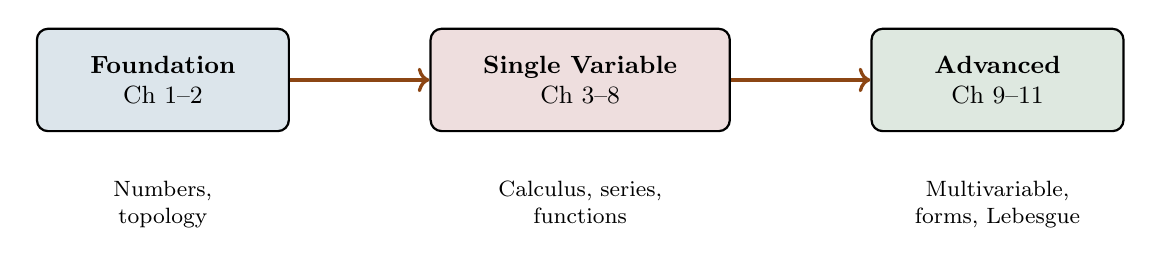
\begin{tikzpicture}[scale=1.0, every node/.style={font=\small}]
    \node[draw, rounded corners, thick, fill=defcolor!15, minimum width=3.2cm, minimum height=1.3cm, align=center] (f) at (0,0) {\textbf{Foundation}\\Ch 1--2};
    \node[draw, rounded corners, thick, fill=thmcolor!15, minimum width=3.8cm, minimum height=1.3cm, align=center] (s) at (5.3,0) {\textbf{Single Variable}\\Ch 3--8};
    \node[draw, rounded corners, thick, fill=proofcolor!15, minimum width=3.2cm, minimum height=1.3cm, align=center] (a) at (10.6,0) {\textbf{Advanced}\\Ch 9--11};
    \draw[->, very thick, mAccent] (f) -- (s);
    \draw[->, very thick, mAccent] (s) -- (a);
    \node[below=0.5cm of f, align=center, text width=3.2cm, font=\footnotesize] {Numbers,\\topology};
    \node[below=0.5cm of s, align=center, text width=3.8cm, font=\footnotesize] {Calculus, series,\\functions};
    \node[below=0.5cm of a, align=center, text width=3.2cm, font=\footnotesize] {Multivariable,\\forms, Lebesgue};
  \end{tikzpicture}
  \end{center}

  \vspace{0.5em}
  \textbf{Eleven chapters, three broad phases.}

  \note{
    The book has eleven chapters that fall naturally into three phases. Chapters 1 and 2 are the foundation, where we build the real numbers and the basic topology of metric spaces. Chapters 3 through 8 are the heart of single-variable analysis, covering sequences, series, continuity, differentiation, integration, and special functions. Chapters 9 through 11 are the advanced material: functions of several variables, differential forms, and a first taste of Lebesgue theory. Let's look at each chapter in a bit more detail.
  }
\end{frame}

% --- Chapters 1--4 ---
\begin{frame}{The Eleven Chapters --- Part 1}
  \begin{enumerate}
    \item The Real and Complex Number Systems
    \item Basic Topology
    \item Numerical Sequences and Series
    \item Continuity
  \end{enumerate}

  \note{
    The book is organized into eleven chapters. The first four form the foundation. Chapter 1 builds the real and complex number systems from the ground up. Chapter 2 introduces the basic topology of metric spaces, including open sets, closed sets, and compactness. Chapter 3 develops the theory of sequences and series of numbers. Chapter 4 uses all of this to give a careful treatment of continuity.
  }
\end{frame}

% --- Chapters 5--8 ---
\begin{frame}{The Eleven Chapters --- Part 2}
  \begin{enumerate}
    \setcounter{enumi}{4}
    \item Differentiation
    \item The Riemann-Stieltjes Integral
    \item Sequences and Series of Functions
    \item Some Special Functions
  \end{enumerate}

  \note{
    Chapters 5 through 8 cover the core of single-variable analysis. Chapter 5 is about differentiation, including the mean value theorem and Taylor's theorem. Chapter 6 develops the Riemann-Stieltjes integral, a flexible generalization of the ordinary Riemann integral. Chapter 7 studies what happens when you take limits of entire sequences of functions, introducing uniform convergence. Chapter 8 applies all of this to special functions like the exponential, logarithm, trigonometric functions, and the gamma function.
  }
\end{frame}

% --- Chapters 9--11 ---
\begin{frame}{The Eleven Chapters --- Part 3}
  \begin{enumerate}
    \setcounter{enumi}{8}
    \item Functions of Several Variables
    \item Integration of Differential Forms
    \item The Lebesgue Theory
  \end{enumerate}

  \note{
    The final three chapters are more advanced. Chapter 9 extends calculus to functions of several variables, including the inverse and implicit function theorems. Chapter 10 develops differential forms and builds up to Stokes' theorem, a deep unifying result. Chapter 11 gives a brief but rigorous introduction to Lebesgue measure and integration, which is the modern foundation of integration theory.
  }
\end{frame}

% ============================================================
\section{Open Source and Contributing}
% ============================================================

% --- Build 1/3 ---
\begin{frame}{This Project is Open Source}
  \begin{defblock}{Open and collaborative}
    The slides, diagrams, and speaker notes for this series are \alert{open source}.
  \end{defblock}

  \note{
    One more important point. The slides, the diagrams, and the speaker notes for this entire series are open source. That means the full source code is publicly available for anyone to read, study, or modify. You can see exactly how each slide was built, and you can reuse the material freely under the project's license.
  }
\end{frame}

% --- Build 2/3 ---
\begin{frame}{This Project is Open Source}
  \begin{defblock}{Open and collaborative}
    The slides, diagrams, and speaker notes for this series are \alert{open source}.
  \end{defblock}

  \vspace{0.5em}
  \textbf{Anyone can contribute:}
  \begin{itemize}
    \item Fix typos and errors
    \item Improve explanations and diagrams
    \item Suggest new insights or alternative proofs
  \end{itemize}

  \note{
    Because the project is open, anyone can contribute. If you spot a typo, a bug in a diagram, or a confusing explanation, you are welcome to send a fix. If you have a better way to visualize an idea, or an alternative proof that you find more illuminating, those contributions are also welcome. The goal is to make this resource better over time, through the collective effort of everyone who uses it.
  }
\end{frame}

% --- Build 3/3 ---
\begin{frame}{This Project is Open Source}
  \begin{defblock}{Open and collaborative}
    The slides, diagrams, and speaker notes for this series are \alert{open source}.
  \end{defblock}

  \vspace{0.5em}
  \textbf{Anyone can contribute:}
  \begin{itemize}
    \item Fix typos and errors
    \item Improve explanations and diagrams
    \item Suggest new insights or alternative proofs
  \end{itemize}

  \vspace{0.5em}
  \alert{Together, we can make learning analysis easier for everyone.}

  \note{
    Together, we can make learning analysis easier for everyone. Mathematics is a shared human project, and the more people who help explain it well, the more accessible it becomes to the next generation of learners. Thank you for being part of that.
  }
\end{frame}

% ============================================================
\section{Let's Begin}
% ============================================================

\begin{frame}{Ready to Start}
  \textbf{What's next:}
  \begin{itemize}
    \item Chapter 1, Section 1: \emph{Introduction}
    \item Why the rationals are not enough
    \item The first glimpse of the real numbers
  \end{itemize}

  \vspace{1em}
  \begin{center}
    \alert{\Large Let's dive in.}
  \end{center}

  \note{
    That is everything you need to know before we start. In the next video, we begin Chapter 1, Section 1, the Introduction. We will see why the rational numbers are not enough for doing analysis, and we will get our first glimpse of the real number system. Grab a copy of Rudin if you can, get comfortable, and let's dive in.
  }
\end{frame}

\end{document}
